\documentclass[oneside, mag]{mgr}	
 
\usepackage{polski}	
\usepackage[utf8]{inputenc}	
\usepackage{amsmath}		
\usepackage{graphicx}	
\graphicspath{ {./} }
\usepackage{amsfonts}
\usepackage{hyperref}
\usepackage{tabstackengine}
\usepackage{caption}
\usepackage{subfig}
\usepackage{listings}
\usepackage{tikz}
\usetikzlibrary{positioning}

\newcommand{\bb}{\textbf}

\title{Analiza efektywności zastosowania sieci rekurencyjnych w zadaniu klasyfikacji}	
\engtitle{Analysis of the effectiveness of recursive networks in the classification task}
\author{Jędrzej Kozal}
\supervisor{dr  inż. Paweł Ksieniewicz}

\field{Informatyka (Inf)}
\specialisation{Systemy informatyki w medycynie (IMT)}

\begin{document}
\bibliographystyle{plabbrv}	

\maketitle

\tableofcontents

\chapter{Wstęp}

W niniejszym rozdziale zarysowano problematykę pracy i pokrótce omówiono zagadnienia, które będą wykorzystywane w dalszej części. Dokonano przeglądu literaturowego i opisano plan badań.

\section{Wprowadzenie}

Sekcji ta zawiera wprowadzenie podstawowych zagadnień, wykorzystywane w pracy, oraz nakreślono rys historyczny badań związanych z tematyką pracy.

\subsection{Sieci neuronowe}

\begin{figure}
	\centering
	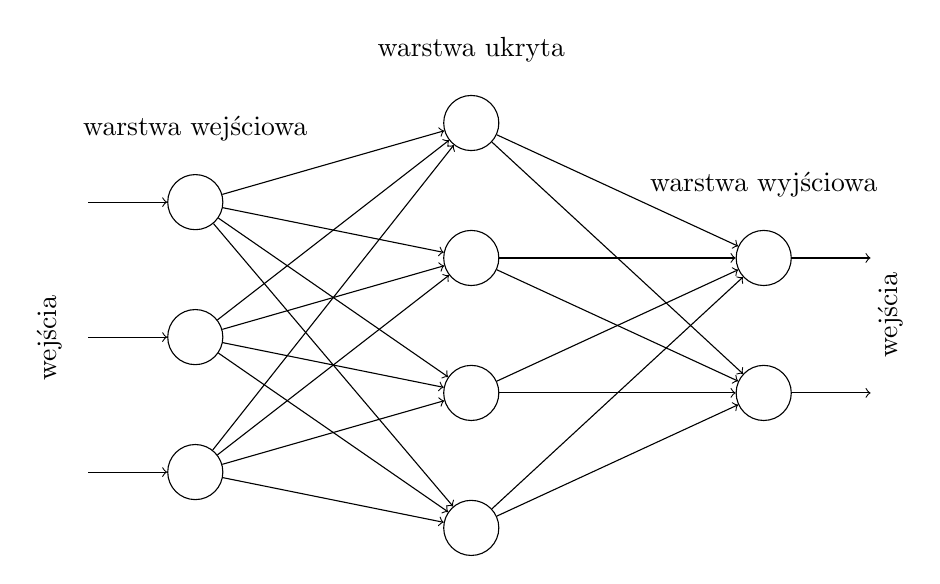
\begin{tikzpicture}[auto,node distance=1.5cm]
	\tikzstyle{node}=[circle,draw]
		\node[node, minimum size=0.7cm, label={[yshift=0.3cm]warstwa wejściowa}] (i1) {$ $};
		\node[node, minimum size=0.7cm] (i2) [below=1.0cm of i1] {$ $};
		\node[node, minimum size=0.7cm] (i3) [below=1.0cm of i2] {$ $};
		\node[node, minimum size=0.7cm, label={[yshift=0.3cm]warstwa ukryta}] (h1) [above right=0.5cm and 3.0cm of i1] {$ $};
		\node[node, minimum size=0.7cm] (h2) [below=1.0cm of h1] {$ $};
		\node[node, minimum size=0.7cm] (h3) [below=1.0cm of h2] {$ $};
		\node[node, minimum size=0.7cm] (h4) [below=1.0cm of h3] {$ $};
		\node[node, minimum size=0.7cm, label={[yshift=0.3cm]warstwa wyjściowa}] (o1) [right= 3.0cm of h2] {$ $};
		\node[node, minimum size=0.7cm] (o2) [below=1.0cm of o1] {$ $};
			\draw[->] (i1) edge node {$ $} (h1);
			\draw[->] (i1) edge node {$ $} (h2);
			\draw[->] (i1) edge node {$ $} (h3);
			\draw[->] (i1) edge node {$ $} (h4);
			\draw[->] (i2) edge node {$ $} (h1);
			\draw[->] (i2) edge node {$ $} (h2);
			\draw[->] (i2) edge node {$ $} (h3);
			\draw[->] (i2) edge node {$ $} (h4);
			\draw[->] (i3) edge node {$ $} (h1);
			\draw[->] (i3) edge node {$ $} (h2);
			\draw[->] (i3) edge node {$ $} (h3);
			\draw[->] (i3) edge node {$ $} (h4);
			\draw[->] (h1) edge node {$ $} (o1);
			\draw[->] (h1) edge node {$ $} (o2);
			\draw[->] (h2) edge node {$ $} (o1);
			\draw[->] (h2) edge node {$ $} (o2);
			\draw[->] (h3) edge node {$ $} (o1);
			\draw[->] (h3) edge node {$ $} (o2);
			\draw[->] (h4) edge node {$ $} (o1);
			\draw[->] (h4) edge node {$ $} (o2);
			\node (input1) [left=1.0cm of i1] {$ $};
			\node[label={[xshift=-0.25cm, yshift=0.65cm, rotate=90]left:wejścia}] (input2) [left=1.0cm of i2] {$ $};
			\node (input3) [left=1.0cm of i3] {$ $};
			\draw[->] (input1) edge node {$ $} (i1);
			\draw[->] (input2) edge node {$ $} (i2);
			\draw[->] (input3) edge node {$ $} (i3);
			\node (output1) [right=1.0cm of o1] {$ $};
			\node[label={[xshift=0.25cm, yshift=1.65cm, rotate=90]left:wejścia}] (output2) [right=1.0cm of o2] {$ $};
			\draw[->] (o1) edge node {$ $} (output1);
			\draw[->] (o2) edge node {$ $} (output2);
\end{tikzpicture}
	\caption{Schemat sieci neuronowej}
	\label{feedforward-NN}
\end{figure}

Sieci neuronowe to szeroka klasa modeli wykorzystywana najczęściej do zadania uczenia nadzorowanego. W podstawowej formie sieć składa się z wielu warstw neuronów połączonych ze sobą (zob rys. \ref{feedforward-NN}). Warstwa wejściowa sieci odpowiada za przyjmowanie wektorów wejściowych. Neurony w warstwie ukrytej realizują funkcję nieliniową opisaną równaniem:

\begin{equation}
	x_i = f(w_i u_i)
\end{equation}

Gdzie $x_i$ jest wyjściem $i$-tego neuronu w warstwie (nazywanym również aktywacją neuronu), $f$ jest funkcją aktywacji w warstwie do której należy neuron, $w_i$ jest wektorem wag $i$-tego neuronu a $u_i$ jest wektorem wejść $i$-tego neuronu. Nieliniowość całej operacji jest powodowana przez nieliniową funkcję aktywacji. W procesie uczenia definiowana jest funkcja strat (ang. loss function) $L$ opisująca w sposób ilościowy jak bardzo wyjście sieci neuronowej różni się od oczekiwanej wartości. Wartości funkcji strat są wykorzystywane do modyfikacji wag sieci neuronowej (algorytm wstecznej propagacji błędu), najczęściej z wykorzystaniem reguł gradientowych. Dzięki algorytmowi wstecznej propagacji możliwe jest uczenie wielowarstwowych sieci. Wyjście każdej warstwy stanowi zmodyfikowaną reprezentację oryginalnej przestrzeni. Przez nieliniowości i tworzenie reprezentacji przestrzeni cech, wielowarstwowe sieci neuronowe posiadają zdolność do generowania bardzo złożonych granice decyzyjne.

Sieci neuronowe są stosunkowo starą klasą modeli. Pierwsze prace w zakresie reguł uczenia pojawiły się latach 40 XX wieku \cite{McCulloch-Pitts} \cite{Hebb}. Rosenblat \cite{Rosenblatt} skonstruował perceptron - maszynę wykazującą zdolność nauki. Uważa się, że publikacja w które zbadano ogarniczenia perpceptoronu i udowodniono, że podejedyncza wartswa sieci nie jest w stanie nauczyć się funkcji XOR \cite{Perceptrons} zaczpoątkowała okres nazwany zimą sztucznej inteligencji (ang. AI Winter). Prawdziwym przełomem okazała się praca \cite{Rumelhart}, w której zaproponowano algorytm wstecznej propagacji błędów. Po publikacji tej zainteresowanie głębokimi sieciami neuronowymi zaczęło wzrastać. W \cite{Conv} zaproponowano warstwy konwolucyjne, które pozwoliły na łatwiejsze przetwarzanie obrazów przez sieci neuronowe. 
Gwałtowny wzrost popularności sieci neuronowych w ostatnich latach można przypisać kilku czynnikom \cite{Goodfellow-et-al-2016}. Pierwszym z nich jest zwiększenie mocy obliczeniowej dostępnej dla praktyków i badaczy uczenia maszynowego, co pozwoliło na zwiększenie rozmiarów modeli i skrócenie czasu uczenia. Drugim czynnikiem jest pojawienie wielu obszernych zbiorów danych, powodowane przez rozpowszechnienie się internetu i urządzeń elektronicznych w życiu codziennym ludzi. Oba te czynniki pozwalają na skuteczne trenowanie modeli o większych pojemnościach, przeznaczonych do coraz bardziej złożonych zadań.

Można dopatrywać się powiązań między sposobem działania ludzkiego mózgu a sieciami neuronowymi. Podobieństwo to może być widoczne w sposobie działania synaps komórki nerowowej. Badacze podkreślają \cite{Goodfellow-et-al-2016}, że związek sieci neuronowych z biologią ma bardziej charakter luźnej inspiracji niż rzeczywistego modelu zjawisk zachodzących w ludzkim mózgu.

\subsection{Rekurencyjne sieci neuronowe}

\begin{figure}
\centering
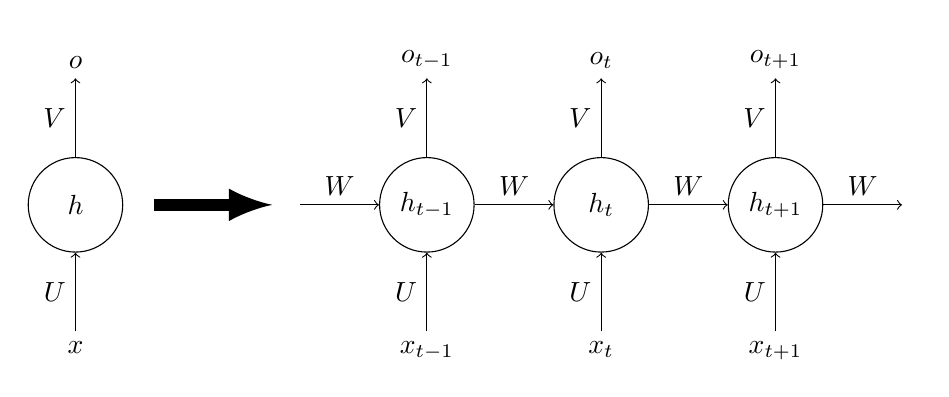
\begin{tikzpicture}[auto,node distance=1.5cm]
	\tikzstyle{node}=[circle,draw]
		\node[node, minimum size=1.2cm] (h) {$h$};
		\node (o) [above=1.0cm of h] {$o$};
		\node (x) [below=1.0cm of h] {$x$};
			\draw[->] (h) edge node {$V$} (o);
			\draw[->] (x) edge node {$U$} (h);
		\node[right=2.0cm of h] (h0) {$ $};
		\node[node, right=1.0cm of h0, minimum size=1.2cm] (ht_1) {$h_{t-1}$};
		\node (ot_1) [above=1.0cm of ht_1] {$o_{t-1}$};
		\node (xt_1) [below=1.0cm of ht_1] {$x_{t-1}$};
			\draw[->] (h0) edge node {$W$} (ht_1);
			\draw[->] (ht_1) edge node {$V$} (ot_1);
			\draw[->] (xt_1) edge node {$U$} (ht_1);
		\node[node, right=1.0cm of ht_1, minimum size=1.2cm] (ht) {$h_{t}$};
		\node (ot) [above=1.0cm of ht] {$o_{t}$};
		\node (xt) [below=1.0cm of ht] {$x_{t}$};
			\draw[->] (ht_1) edge node {$W$} (ht);
			\draw[->] (ht) edge node {$V$} (ot);
			\draw[->] (xt) edge node {$U$} (ht);
		\node[node, right=1.0cm of ht, minimum size=1.2cm] (ht1) {$h_{t+1}$};
		\node (ot1) [above=1.0cm of ht1] {$o_{t+1}$};
		\node (xt1) [below=1.0cm of ht1] {$x_{t+1}$};
			\draw[->] (ht) edge node {$W$} (ht1);
			\draw[->] (ht1) edge node {$V$} (ot1);
			\draw[->] (xt1) edge node {$U$} (ht1);
		\node (hend) [right=1.0cm of ht1] {$ $};
			\draw[->] (ht1) edge node {$W$} (hend);
			\pgfsetarrowsend{latex} 
			\pgfsetlinewidth{1ex} 
			\pgfpathmoveto{\pgfpoint{1.0cm}{0.0cm}} 
			\pgfpathlineto{\pgfpoint{2.5cm}{0.0cm}} 
			\pgfusepath{stroke} 
			\useasboundingbox (-0.25,-0.25) rectangle (3.75,2.25);
\end{tikzpicture}
\caption{Schemat sieci rekurencyjnej.} (Lewo) sieci rekurencyjne można przedstawić jako jednostkę obliczeniową, która do realizacji obliczeń wykorzystuje wartości uzyskane dla poprzednich kroków. Na rysunku jest to widoczne w formie czarnego kwadratu, oznaczającego opóźnienie czasowe o jeden krok przy neuronie obok normalnych wejść i wyjść. (Prawo) rozwinięta wersja tego samego schematu, przedstawiająca w jaki sposób obliczenia są wykonywane w poszczególnych krokach. Reprezentacja ta pozwala na łatwiejszą analizę zachowań sieci i stosowanych algorytmów. 
	\label{fig:rnn}
\end{figure}


Sieci feedforward posiadają stałą liczbę wejść i wyjść, przez co nie radzą sobie dobrze z przetwarzaniem danych występujących w ciągach (takich jak tekst, dźwięki czy ciągi czasowe). Istnieją podejścia umożliwiające przetwarzanie ciągów przez sieci feedforward, ale nie cechują się wysoką skutecznością. W celu zaadresowania tego problemu powstały sieci rekurencyjne (ang. Recurrent Neural Networks - RNN).
Sieci Rekurencyjne zostały oparte na pracy Rumelharta \cite{RNN}. RNN posiadają ukryty stan, będący wektorem przekazywanym między poszczególnymi krokami czasowymi. Stan jest obliczany przez warstwą ukrytą sieci, której wartość jest obliczana nie tylko na podstawie aktualnego wejścia, ale też na podstawie poprzedniego stanu sieci (zob rys. \ref{fig:rnn}).
Algorytm uczenia RNN - propagacja wsteczna w czasie (ang. Back-Propagation Through Time - BPTT) została przedstawiona w \cite{BPTT}.
Udowodniono, że przy pewnych założeniach RNN są kompletne w sensie Turinga \cite{turing-complete}.

\subsubsection{Sieci dwukierunkowe}

Wprowadzono wiele modyfikacji w zakresie zasad działania i strukturze RNN. 
W \cite{bidirectional} wprowadzono sieci dwukierunkowe przetwarzające sekwencje w dwóch kierunkach: od początku do końca i od końca do początku. Ostateczna wartość aktywacji dla n-tego elementu sekwencji jest obliczana na podstawie n-tych aktywacji dla obu kierunków.

\subsubsection{LSTM}

RNN w swojej natywnej formie nie są w stanie nauczyć się długich zależności w ciągu uczącym. Problem ten jest w znacznej mierze spowodowany wybuchającymi lub znikającymi gradientami (exploding or vanishing gradients) \cite{vanishing_gradient_RNN}. W celu zaadresowania tego problemu Hochreiter i Schmidhuber zaproponowali architekturę Long Short-Term Memory (LSTM) \cite{LSTM}. Ze względu na swoją strukturę LSTM jest w stanie operować na danych z długimi zależnościami czasowymi. LSTM została dokładniej opisana w dalszej części pracy. 

\subsubsection{GRU}

Gated Recurrent Unit (GRU) \cite{DBLP:journals/corr/ChoMGBSB14} jest modyfikacją LSTM. W wyniku zastosowanych uproszeńw strukturze komórki GRU wymaga mniejszej mocy obliczeniowej do treningu, kosztem mniej mocy modelu. LSTM i GRU uzyskują porównywalne wyniki w praktycznych zastosowaniach \cite{DBLP:journals/corr/ChungGCB14}. GRU została dokładniej opisana w dalszej części pracy.

\subsubsection{Neuronowe Maszyny Turinga}

Rozwinięciem idei wykorzystania pamięci do usprawnienia działania sieci rekurencyjnej są Neuronowe Maszyny Turinga \cite{DBLP:journals/corr/GravesWD14}. Neuronowe Maszyny Turinga korzystają z mechanizmu uwagi do wykonywania operacji na pamięci. Pamięć wykorzystana w tym modelu przypomina pamięć dostępną w komputerze i składa się z wielu wektorów, które można wykorzystać do odczytywania lub przechowywania informacji. Neuronowa Maszyna Turinga posiada dwie głowice: do zapisu i odczytu. Adresowanie pamięci odbywa się na podstawie zawartości (content-base addressing) lub położenia (location-base addressing). Jest to bardzo interesująca klasa modeli, która często posiada bardzo złożone grafy obliczeniowe. Ze względu na ograniczoną dostępną moc obliczeniową do przeprowadzenia badań Neuronowe Maszyny Turinga nie zostały wykorzystane w eksperymentach.

\subsection{Zadanie klasyfikacji}

Uczenie nadzorowane (ang. supervised learning) to dział uczenia maszyn w którym zbiór uczący składa się z par $\{x, d\}_{i=1}^N$, gdzie $x$ to wektor cech, $d$ to etykieta, a $N$ to liczność zbioru uczącego. W przypadku gdy każdej cechy istnieje osobna etykieta mówimy o silnym etykietowaniu. Gdy jedna etykieta opisuje wszystkie cechy z przykładu uczącego mówimy o słabym etykietowaniu. Przykładowo jeśli zadanie polega na rozpoznaniu samochodu na zdjęciu, mówimy o słabym etykietowaniu. Jeśli zadanie polega na zaznaczeniu wszystkich pikseli przedstawiających samochód na zdjęciu, mówimy o silnym etykietowaniu. Aby określić jakość działania algorytmu wprowadza się funkcję straty dla całego zbioru:

\begin{equation}
	\mathcal{L} = \sum_{i=1}^N L_i
\end{equation}

gdzie $L_i$ to wartość funkcji strat do pojedynczego przykładu uczącego. Zadanie klasyfikacji opiera się na przypisaniu przykładu uczącego $x$ do odpowiedniej klasy $k$. W procesie uczenia wybieramy hipotezę z przestrzeni hipotez $h \in \mathcal{H}$, która minimalizuje liczbę błędnie zaklasyfikowanych przykładów \cite{introduction-to-machine-learning}. Można to zapisać za pomocą 0-1 funkcji strat:

\begin{equation}
	E(x, d) = \sum_{i=1}^N 1(h(x_i) \neq d_i )
\end{equation}

gdzie $1(x)$ jest równe 1, gdy x jest prawdziwe i 0 gdy x nie jest prawdziwe. 0-1 funkcja strat może być stosowana, gdy na wyjściu klasyfikatora znajduje się etykieta klasy. W przypadku gdy na wyjściu modelu znajduje się prawdopodobieństwo przynależności do klasy często stosowaną funkcją strat jest entropia krzyżowa (ang. cross entropy):

\begin{equation}
	H(h,d) = - \sum h(x) log(d)
\end{equation}

Reguła decyzyjna w takim przypadku opiera się na wyborze najbardziej prawdopodobnej klasy:

\begin{equation}
	h(x) = arg \; \stackunder{max}{k} \; p(C_k | x)
\end{equation}

gdzie $x_i$ to $i$-ty element wektora, będącego argumentem funkcji softmax.

W przypadku sieci neuronowych często stosowaną mechaniką jest wykorzystywanie funkcji softmax w warstwie wyjściowej sieci. Funkcja softmax pozwala na konwertowanie wyjść sieci na prawdopodobieństwa i jest dana wzorem:

\begin{equation}
	softmax(x)_i = \frac{e^{x_i}}{\sum_{k=1}^{K} e^{x_k}}
\end{equation}

Algorytmy klasyfikacji dostosowane dla sieci rekurencyjnych takie jak Connectionist Temporal
Classification zostały szczegółowo omówione w \cite{graves-phd}. W przypadku tej pracy ich wymaganie nie będzie wskazane, ze względu na charakter wykorzystanej architektury sieci.

\section{Przegląd literatury}

W tej sekcji dokonano przeglądu typowych zastosowań sieci rekurencyjnych oraz omówiono prace, w których dokonywano klasyfikacji obrazów za pomocą RNN.

\subsection{Zastosowania rekurencyjnych sieci neuronowych}

Sieci Rekurencyjne znalazły wiele zastosowań w przetwarzaniu sekwencji. 
Jednym z takich zastosowań może być przetwarzanie języka naturalnego (natural language processing - NLP), gdzie RNN znalazły zastosowanie w rozpoznawaniu mowy \cite{DBLP:journals/corr/abs-1303-5778}, \cite{speech_recognition}, \cite{speech_recognition1}, tłumaczeniu \cite{translate}, \cite{DBLP:journals/corr/ChoMGBSB14}, \cite{DBLP:journals/corr/BahdanauCB14}, \cite{DBLP:journals/corr/WuSCLNMKCGMKSJL16}, modelowniu języka \cite{DBLP:journals/corr/ChoMGBSB14}, generowaniu mowy \cite{DBLP:journals/corr/MehriKGKJSCB16} i generowaniu tekstu \cite{DBLP:journals/corr/Graves13} \cite{karpathy_RNN_blog}. 
Innym polem zastosowań RNN jest rozpoznawanie pisma ręcznego \cite{handwriting_recognition}, \cite{handwriting_recognition2} lub jego generacja \cite{DBLP:journals/corr/Graves13}.
RNN są także wykorzystywane do generowania obrazów \cite{DBLP:journals/corr/GregorDGW15} i muzyki \cite{DBLP:journals/corr/abs-1804-07300}.
Autorzy \cite{DBLP:journals/corr/VinyalsL15} zaproponowali system do przeprowadzania rozmów zbudowany z wykorzystaniem RNN. 
W \cite{sentiment_analysis} wykorzystano RNN do analizy sentymentu.

Sieci rekurencyjne są także wykorzystywane w połączeniu z innymi modelami np. w połączeniu z CNN w celu generowania podpisów dla obrazów \cite{DBLP:journals/corr/VinyalsTBE14}, gdzie CNN jest wykorzystywane do klasyfikacji obrazu i przygotowywania reprezentacji obrazu w architekturze encoder-decoder, a RNN generuje podpis obrazka.

\subsection{Zastosowanie sieci rekurencyjnych do klasyfikacji obrazów}

W \cite{DBLP:journals/corr/VisinKCMCB15} wykorzystano sieć rekurencyjną do klasyfikacji obrazów. Proponowany model ReNet wykorzystuje RNN do czterotnego trawersowania fragmentów obrazu w celu ekstrakcji cech, jako alternatywę dla warstw konwolucyjnych z poolingiem. W \cite{DBLP:journals/corr/abs-0705-2011} wprowadzono wielowymiarowe sieci rekurencyjne, które obliczały aktywację w danej komórce nie tylko na podstawie aktywacji z poprzedniej iteracji, ale także na podstawie wartości aktywacji sąsiadujących komórek w aktualnym kroku czasowym. Model wielowymiarowych RNN został wykorzystany w przypadku tej pracy do przeprowadzenia segmentacji obrazu. Idea ta została rozwinięta w \cite{DBLP:journals/corr/KalchbrennerDG15}, gdzie przedstawiono Grid LSTM, które rozszerzało standardowy model sieci LSTM do N-wymiarowych komórek ze współdzielonymi wektorami stanu i pamięci. Wielowymiarowe sieci rekurencyjne stanowią ciekawą klasę modeli, mogą jednak wymagać znaczących zasobów mocy obliczeniowej do przeprowadzenia procesu uczenia.

\section{Cel pracy}

Celem pracy jest zbadanie skuteczności klasyfikacji zmodyfikowanej architektury ReNet. Proponowana modyfikacja polega na zastąpieniu czterech sieci rekurencyjnych dwiema sieciami rekurencyjnymi analizącymi obraz skonwertowany do jednowymiarowego ciągu otrzymanego z wykorzystaniem krzywych wypełniającej przestrzeń (ang. space-filling curves). Wyniki klasyfikacji wybranego zbioru danych zostaną porównane z oryginalną architekturą oraz wynikami osiąganymi dla sieci konwolucyjnych. Wykorzystanie dwóch sieci rekurencyjnych zamiast czterech powinno pozwolić na zmniejszenie liczby parametrów modelu. Mniejsza liczba parametrów może przekładać się na krótszy czas szkolenia i może pozwolić wykorzystanie modelu z większą liczbę neuronów w warstwach ukrytych modelu. Modyfikacja sieci będzie mieć wpływ na zdolność uczenia sieci, co oczywiście jest najciekawszym przedmiotem badań. W zakres eksperymentów będzie wchodziło również zbadanie wpływu różnych architektur sieci rekurencyjnych na uzyskiwane wyniki. Ze względu na ograniczoną dostępną moc obliczeniową hiperparametry modeli zostaną dobrane z wykorzystaniem podziału zbioru danych na zbiór uczący i zbiór testowy oraz wykorzystaniem algorytmu wyszukiwania sieciowego (ang. grid search). Dokładność klasyfikacji zostanie zmierzona z wykorzystaniem dokładności (ang. accuracy).




\chapter{Omówienie wybranych zagadnień teoretycznych}

W niniejszym rozdziale zostały omówione teoretyczne podstawy wybranych algorytmów i struktur sieci, które zostały wykorzystane w badaniach.

\section{Rekurencyjna Sieć Neuronowa}

Sieci rekurencyjne są modyfikacją zwykłych sieci feedforward powstałą poprzez dopuszczenie możliwości powstawania cykli w grafie obliczeniowym. Aktywacja każdej jednostki może być wyrażona jako:


\begin{equation}
	h_t = f(h_{t-1}, x_t)
	\label{eq:basic-rnn}
\end{equation}

gdzie $h_t$ to aktywacja jednostki w czasie $t$, $x_t$ to wejście jednostki w czasie $t$, a $f$ oznacza nieliniowe przekształcenie realizowane przez jednostkę obliczeniową. Tego typu sformułowanie zasady działania modelu jest realizacją współdzielenia parametrów przez części modelu. Każda jednostka do obliczenia aktywacji wykorzystuje aktualne wejście i aktywację z poprzedniego kroku. Aby uniezależnić model od długości sekwencji w każdym kroku wykorzystuje się ten sam zestaw parametrów.

W trakcie uczenia sieci dokonuje się rozwinięcia (ang. unfolding) grafu obliczeniowego, poprzez wielokrotne zastosowanie definicji sieci. Przykładowo dla dwóch kroków w czasie odwinięcie grafu można zapisać jako:

\begin{equation}
	h_2 = f(h_1, x_2) = f(f(h_0, x_1), x_2)
\end{equation}

Co jest zastosowaniem równania \ref{eq:basic-rnn} rekurencyjnie $n$ razy. Jako $h_0$ najczęściej stosowany jest wektor zer. Rozwinięcie grafu pozwala na zamianę grafu cyklicznego na acykliczny, bardziej przypominający graf sieci feedforward:

\begin{figure}[!h]
\centering
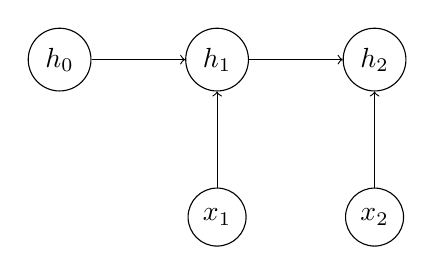
\begin{tikzpicture}[auto,node distance=2.0cm]
	\tikzstyle{node}=[circle,draw]
		\node[node] (h0) {$h_0$};
		\node[node] (h1) [right of=h0] {$h_1$};
		\node[node] (x1) [below of=h1] {$x_1$};
		\node[node] (h2) [right of=h1] {$h_2$};
		\node[node] (x2) [below of=h2] {$x_2$};
			\draw[->] (h0) edge node {$ $} (h1);
			\draw[->] (x1) edge node {$ $} (h1);
			\draw[->] (h1) edge node {$ $} (h2);
			\draw[->] (x2) edge node {$ $} (h2);
\end{tikzpicture}
\end{figure}

Rozwinięty graf pozwala na zastosowanie reguł propagacji wstecznej i obliczenie gradientów funkcji strat. Jest więc to proces umożliwiający uczenie sieci rekurencyjnej.

\begin{figure}
\centering
	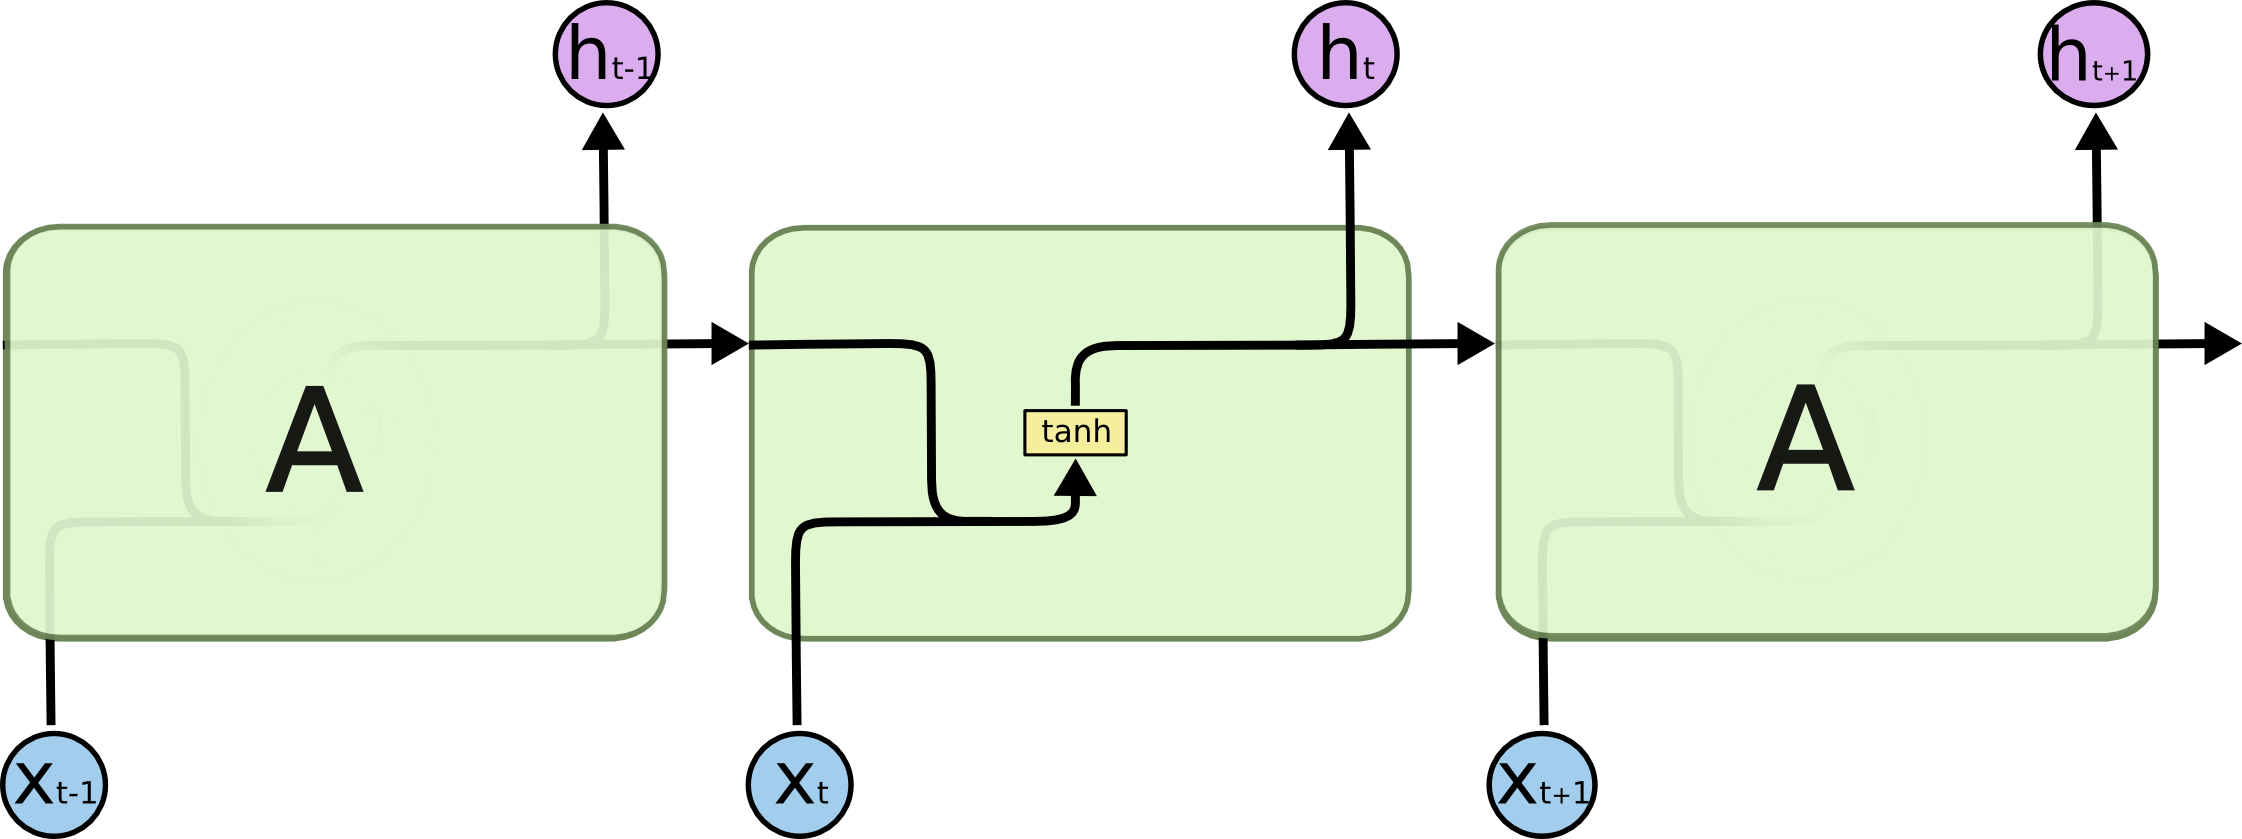
\includegraphics[width=0.9\textwidth]{img/LSTM3-SimpleRNN.png}
	\caption{Schemat podstawowej jednostki sieci rekurencyjnej, korzystającej z funkcji aktywacji $tanhh$.} Źródło: http://colah.github.io/posts/2015-08-Understanding-LSTMs/
	\label{fig:simple_rnn}
\end{figure}

Przekształcenie realizowane przez pojedynczą jednostkę rnn w najbardziej podstawowej formie można zapisać jako:

\begin{equation}
	h_t = g(W h_{t-1} + U x_t + b)
\end{equation}

gdzie $W$ i $U$ to macierze wag i wektor, $b$ to wektor biasu, a $g$ to funkcja aktywacji. Najczęściej stosowanymi funkcjami aktywacji są funkcja sigmoidalna, tanh lub ReLU. Istnieje wiele modyfikacji wprowadzonych do struktury jednostki sieci rekurencyjnej, które zostały omówione w dalszej części rozdziału.

\section{Propagacja wsteczna w czasie}

Propagacja wsteczna w czasie to algorytm dedykowany do uczenia sieci rekurencyjnych. Polega on na wykorzystaniu rozwiniętej formy grafu obliczeniowego sieci rekurencyjnej i zastosowaniu propagacji wstecznej, z uwzględnieniem tego, że każda jednostka rekurencyjna operuje na tym samym zestawie parametrów.

\begin{figure}
\centering
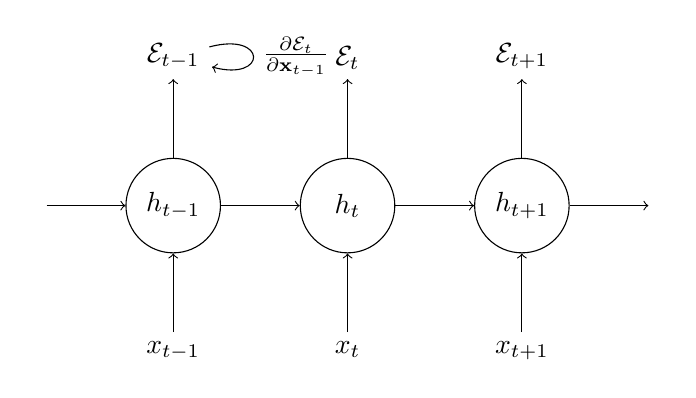
\begin{tikzpicture}[auto,node distance=1.5cm]
	\tikzstyle{node}=[circle,draw]
		\node (h) {$ $};
		\node[node, right=1.0cm of h, minimum size=1.2cm] (ht_1) {$h_{t-1}$};
		\node (ot_1) [above=1.0cm of ht_1] {$\mathcal{E}_{t-1}$};
		\node (xt_1) [below=1.0cm of ht_1] {$x_{t-1}$};
			\draw[->] (h) edge node {$ $} (ht_1);
			\draw[->] (ht_1) edge node {$ $} (ot_1);
			\draw[->, loop right] (ot_1) edge node {$\frac{\partial \mathcal{E}_{t}}{\partial \bb{x}_{t-1}}$} (ht_1);
			\draw[->] (xt_1) edge node {$ $} (ht_1);
		\node[node, right=1.0cm of ht_1, minimum size=1.2cm] (ht) {$h_{t}$};
		\node (ot) [above=1.0cm of ht] {$\mathcal{E}_{t}$};
		\node (xt) [below=1.0cm of ht] {$x_{t}$};
			\draw[->] (ht_1) edge node {$ $} (ht);
			\draw[->] (ht) edge node {$ $} (ot);
			\draw[->] (xt) edge node {$ $} (ht);
		\node[node, right=1.0cm of ht, minimum size=1.2cm] (ht1) {$h_{t+1}$};
		\node (ot1) [above=1.0cm of ht1] {$\mathcal{E}_{t+1}$};
		\node (xt1) [below=1.0cm of ht1] {$x_{t+1}$};
			\draw[->] (ht) edge node {$ $} (ht1);
			\draw[->] (ht1) edge node {$ $} (ot1);
			\draw[->] (xt1) edge node {$ $} (ht1);
		\node (hend) [right=1.0cm of ht1] {$ $};
			\draw[->] (ht1) edge node {$ $} (hend);
\end{tikzpicture}
\caption{Schemat działania propagacji wstecznej w czasie.}
	\label{fig:rnn}
\end{figure}

\begin{equation}
	\mathcal{E}_t = \mathcal{L}(x_t)
\end{equation}

\begin{equation}
	\frac{\partial \mathcal{E}}{\partial \Theta} = \sum_{1 <= t <= T} \frac{\partial \mathcal{E}_t}{\partial \Theta}
\end{equation}

\begin{equation}
	\frac{\partial \mathcal{E}_t}{\partial \Theta} = \sum_{1 <= k <= t} (\frac{\partial \mathcal{E}_t}{\partial \bb{x}_t} \frac{\partial \bb{x}_t}{\partial \bb{x}_k} \frac{\partial \bb{x}_k}{\partial \Theta})
\end{equation}

\begin{equation}
	\frac{\partial \bb{x}_t}{\partial \bb{x}_k} = \prod_{t >= i > k} \frac{\partial \bb{x}_i}{\partial \bb{x}_{i-1}} = \prod_{t >= i > k} \bb{W}^{T}_{rec} diag(\sigma'(\bb{x}_{i-1}))
\end{equation}

\section{LSTM}

\begin{figure}
\centering
	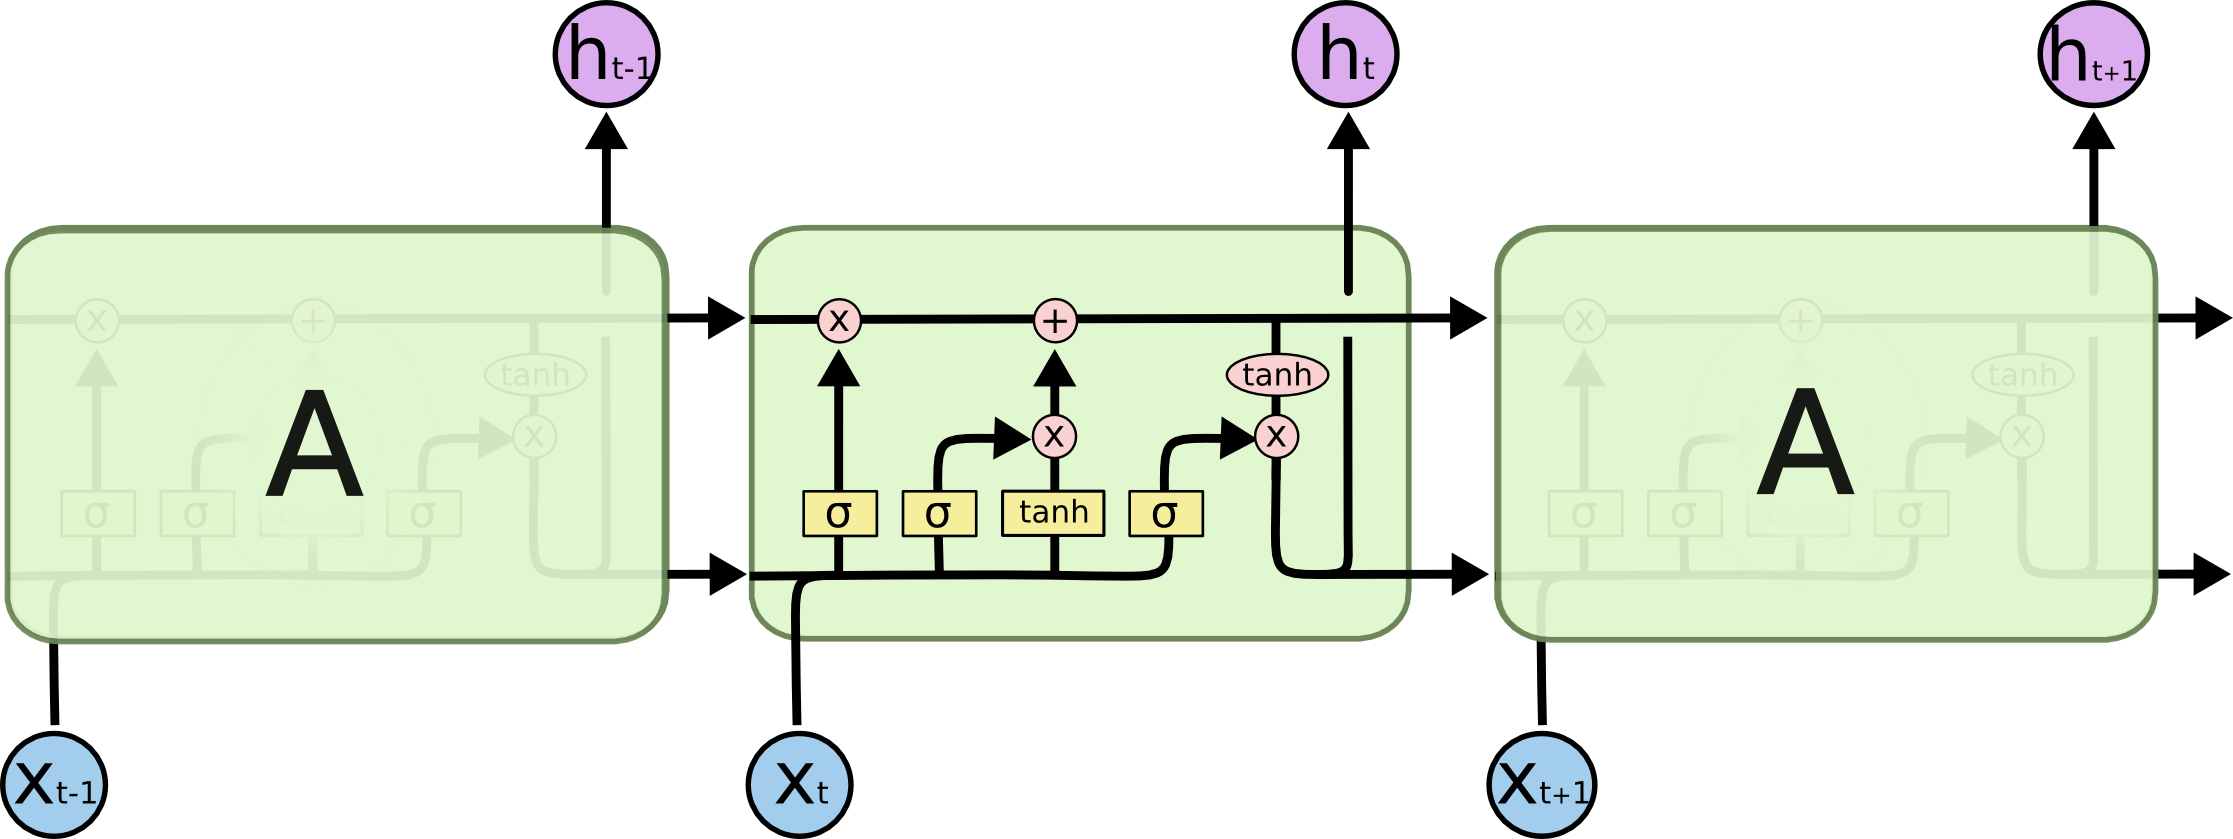
\includegraphics[width=0.90\textwidth]{img/lstm_colah.png}
	\caption{Schemat komórki LSTM.} Źródło: http://colah.github.io/posts/2015-08-Understanding-LSTMs/
	\label{fig:lstm}
\end{figure}

LSTM jest jedną z popularniejszych architektur RNN. Hochreiter i Schmidhuber zaproponowali architekturę Long Short-Term Memory (LSTM) \cite{LSTM} w 1997. Zwykła sieć RNN składa się jedynie ze stanu sieci $h$, oraz wejścia $x$, które są wejściem warstwy ukrytej sieci. Wyjście warstwy ukrytej jest wyjściem sieci. Struktura komórki LSTM jest bardziej skomplikowana i składa się z wektora stanu sieci $h$, komórki pamięci $C$, oraz czterech ukrytych warstw sieci. Schemat ze strukturą sieci został przedstawiony na rys. \ref{fig:lstm}.

Warstwy sieci LSTM z sigmoidalnymi funkcjami aktywacji są nazywane bramkami multiplikatywnymi. Sigmoidalna funkcja aktywacji jest opisywana za pomocą wzoru:

\begin{equation}
	\sigma(x) = \frac{1}{e^{-x} + 1}
\end{equation}

i posiada zbiór wartości $(0, 1)$. Przemnożenie wyjścia tej warstwy z dowolną wartością powoduje jej przeskalowanie, przez co warstwy te są wykorzystywane do kontrolowania wartości zmiennych komórki LSTM. Dodatkowo bramki jako warstwy sieci posiadają wagi, które ulegają modyfikacji w trakcie uczenia, przez co LSTM w procesie uczenia zyskują informację o tym kiedy i w jaki sposób uaktualnić swój stan i komórkę pamięci na podstawie obecnie posiadanych informacji. Wyróżnia się 3 bramki. Pierwszą z nich jest forget gate. Jest ona odpowiedzialna za zmniejszanie wartości aktualnie znajdującej się w komórce pamięci. Operacja realizowana przez forget gate jest opisywana wzorem: 

\begin{equation}
	f_t = \sigma( W_f [ h_{t-1}, x_t ] + b_f )
\end{equation}

Gdzie $W_f$ i $b_f$ to odpowiednio wagi i bias warstwy, $h_{t-1}$ to stan komórki z poprzedniego kroku, a $x_t$ to aktualne wejście sieci. Kolejną bramką jest input gate. Realizowana operacja wyraża się analogicznym wzorem:

\begin{equation}
	i_t = \sigma( W_i [ h_{t-1}, x_t ] + b_i )
\end{equation}

Intuicyjnie jest ona odpowiedzialna za określanie w jakim stopniu należy zaktualizować komórkę pamięci sieci na podstawie aktualnego wejścia sieci $x_t$ i stanu z poprzedniego kroku $h_{t-1}$. Na podstawie $x_t$ i $h_{t-1}$ jest obliczana wartość $\tilde{C}_t$:

\begin{equation}
	\tilde{C}_t = tanh( W_c [ h_{t-1}, x_t ] + b_C )
\end{equation}

Wartość $\tilde{C}_t$ może być określona jako kandydat do zastąpienia stanu komórki z poprzedniego kroku $C_{t-1}$. Aktualna wartość $C_t$ jest zatem obliczana ze wzoru:

\begin{equation}
	C_t = f_t \odot C_{t-1} + i_t \odot \tilde{C}_t
\end{equation}

gdzie $\odot$ oznacza iloczyn Hadamarda (iloczyn wszystkich odpowiadających sobie elementów wektora lub macierzy). Ostatnią bramką jest output gate. Realizowana operacja jest dana wzorem:

\begin{equation}
	o_t = \sigma( W_o [ h_{t-1}, x_t ] + b_o )
\end{equation}

Bramka ta służy do określania sposobu w jaki zostanie zaktualizowany stan $h$ w aktualnym kroku $t$, co wyraża się równaniem:

\begin{equation}
	h_t = o_t \odot tanh( C_t )
\end{equation}

\begin{figure}
\centering
	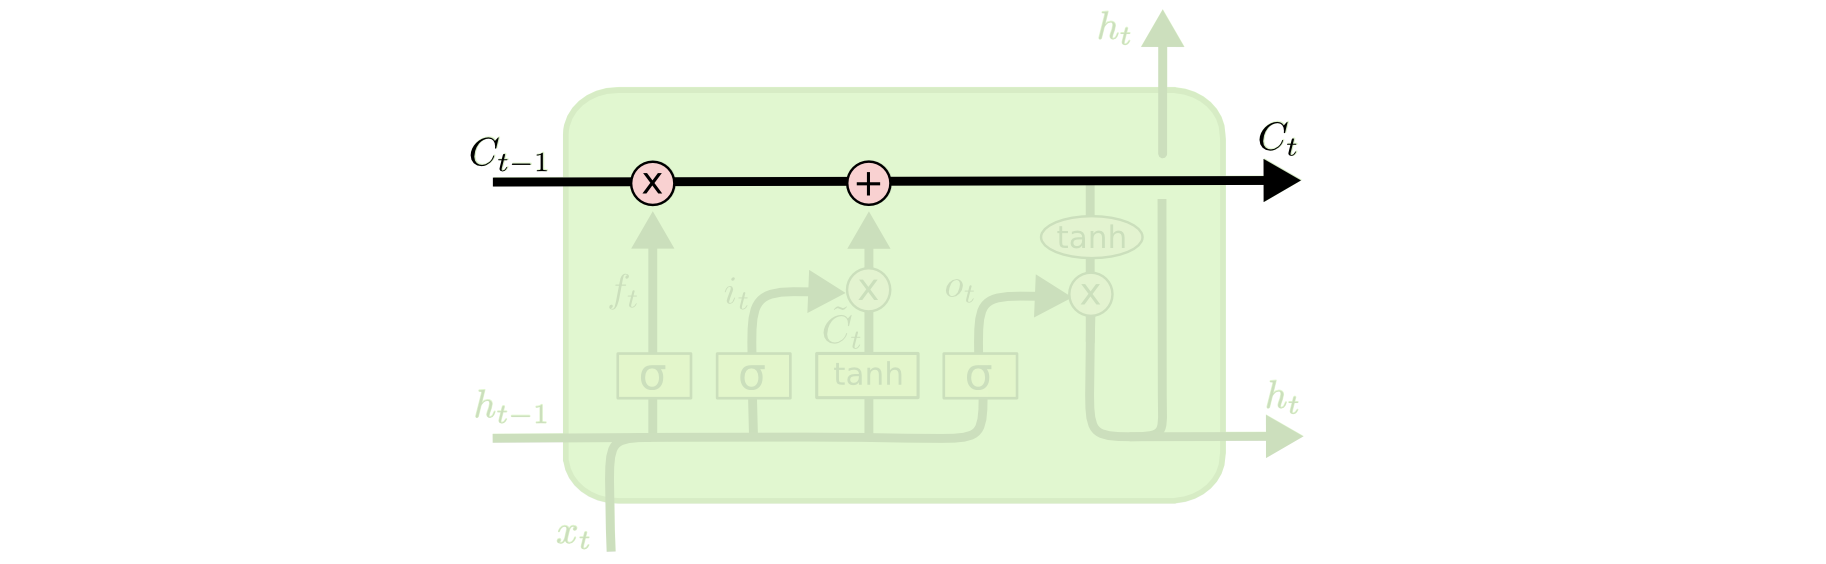
\includegraphics[width=0.90\textwidth]{img/LSTM3-C-line.png}
	\caption{Schemat komórki LSTM z zaznaczoną komórką pamięci.} Źródło: http://colah.github.io/posts/2015-08-Understanding-LSTMs/. W przypadku propagacji wstecznej przy cofaniu się przez graf obliczeniowy sieci węzły odpowiadające operacji dodawania propagują wartość błędu bez modyfikacji wartości. Węzły w grafie odpowiadające operacji mnożenia powodują przemnożenie wartości dotychczasowego błędu przez drugi argument. W tym przypadku realizowana operacja to $C_t = f_t \odot C_{t-1} + i_t \odot \tilde{C}_t$. W wyniku propagacji wstecznej uzyskujemy pochodną $\frac{\partial L}{\partial C_t}$. Opearcja dodawnia nie zmienia wartość błędu, więc $\frac{\partial L}{\partial (f_t \odot C_{t-1})} = \frac{\partial L}{\partial C_t}$. Przy operacji mnożenia pochodna cząstkowa względem $C_{t-1}$ wynosi $\frac{\partial C_t}{\partial C_{t-1}} = f_t$. Błąd propagowany przez komórkę pamięci ma ostateczną wartość: $\frac{\partial L}{\partial C_{t-1}} = \frac{\partial L}{\partial C_t} f_t$. Ze względu na zbiór wartości funkcji sigmoidalnej $f_t \in (0, 1)$ wartość propagowanego błędu nadal jest pomniejszana w każdym kroku. Intuicyjnie wartość błędu jest zmniejszana w takim samym stopniu jak wartość sygnału przy normalnym przejściu przez forget gate (decyzja w jakim stopniu informacje nie są istotne w aktualnym kontekście). Zaproponowana architektura unika jednakże obliczania pochodnej względem funkcji aktywacji sigmoidalnej (pochodna funkcji sigmoidalnej: $\frac{d \sigma}{dx} = \sigma (x)(1 - \sigma (x)$) przy propagacji wstecznej błędu, co powoduje wolniejsze zmniejszanie wartości sygnału błędu. 
	\label{fig:lstm-mem-cell}
\end{figure}

Warto zwrócić uwagę, że w powyższym równaniu nie występują wagi ani bias, więc $tanh$ nie jest utożsamiony z warstwą sieci neuronowej.

W swojej pracy \cite{LSTM} Hochreiter i Schmidhuber odnoszą się do wcześniejszej pracy \cite{vanishing_gradient_RNN}, gdzie zostały przeanalizowane źródła problemów związanych ze znikającymi gradientami. Jako główny problem został wskazany gradient względem dowolnej zmiennej $a$ w grafie obliczeniowym $|\frac{\partial L}{\partial a}| > 1.0$ powodujący wybuchanie wag, lub $|\frac{\partial L}{\partial a}| < 1.0$ powodujący znikanie wag. W strukturze LSTM komórka pamięci jest sposobem zapobiegania temu problemowi. Komórka pamięci przy propagacji wstecznej pozwala na swobodniejszą propagację błędu wiele kroków wstecz, dzięki czemu sieć w procesie uczenia jest w stanie uwzględnić długie zależności czasowe (zob rys. \ref{fig:lstm-mem-cell}). Kolejnym problemem związanym z uczeniem zwykłych RNN jest otrzymywanie sprzecznych sygnałów przy aktualizacji wag. W trakcie uczenia ta sama warstwa sieci jest odpowiedzialna za określenie w jakim stopniu stan sieci z poprzedniego kroku jest nadal istotny, oraz w jakim stopniu można wykorzystać aktualną wartość stanu sieci do obliczenia aktywacji komórki. W tym przypadku uczenie sieci może być trudne. W LSTM ten problem został rozwiązany przez wyodrębnienie bramek i warstw odpowiedzialnych za osobne operacje.  

\section{GRU}

\begin{figure}
\centering
	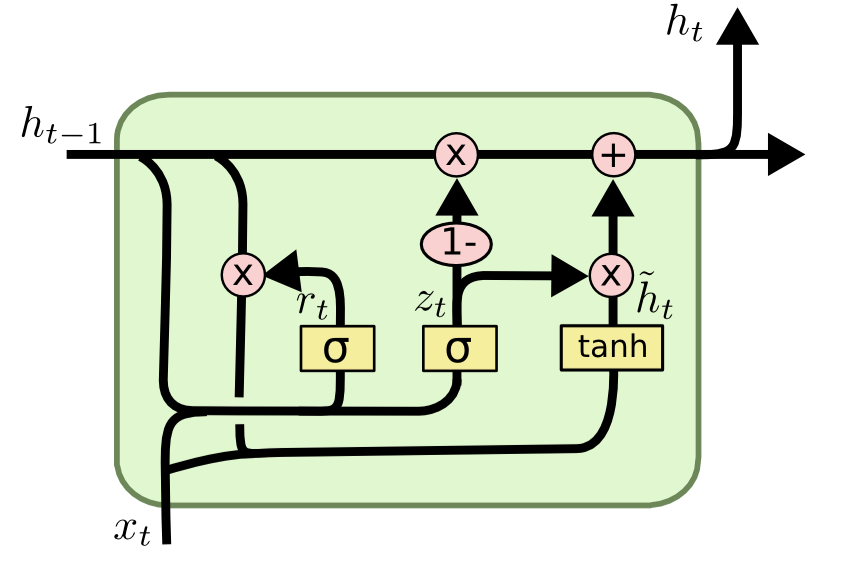
\includegraphics[width=0.5\textwidth]{img/LSTM3-var-GRU.png}
	\caption{Schemat komórki GRU.} Źródło: http://colah.github.io/posts/2015-08-Understanding-LSTMs/
	\label{fig:gru}
\end{figure}

Struktura komórki Gated Reccurent Unit (GRU) została wprowadzona w \cite{DBLP:journals/corr/ChoMGBSB14}. Komórka GRU w znacznym stopniu przypomina strukturę komórki LSTM. GRU również wykorzystuje bramki multiplikatywne do obliczania wartości stanu ukrytego w kolejnych krokach czasowych. Znacząca różnica polega na zastosowaniu dwóch bramek zamiast trzech, pełniących inne funkcje. Ciąg operacji realizowanych przez bramki i warstwy ukryte GRU omówiono poniżej.

Pierwsza bramka stosowana w ciągu przekształceń to reset gate, której aktywacje są obliczane jako:

\begin{equation}
	r_t = \sigma (W_r x_t + U_r h_{t-1})
\end{equation}

gdzie $W_r$ i $U_r$ są macierzami wag skojarzonymi z reset gate, $x$ oznacza wejście komórki a $h_{t-1}$ oznacza stan z poprzedniego kroku. Na podstawie $r$ obliczana jest wartość $\tilde{h_t}$:

\begin{equation}
	\tilde{h_t} = tanh(Wx_t + U(r_t \odot h_{t-1})
\end{equation}

gdzie $W$ i $U$ oznaczają skojarzone z operacją macierze wag, a $\tilde{h_t}$ oznacza kandydata do zastąpienia wektora stanu z poprzedniego kroku $h_{t-1}$. Intuicyjnie można powiedzieć, że reset gate ma za zadanie określić w jakich sytuacjach poprzedni stan sieci zawiera istotne informacje biorąc pod uwagę wejście w danym kroku. Jeśli $r_t$ będzie miało wartość bliską 0, $\tilde{h_t}$ będzie obliczone głównie na podstawie aktualnego wejścia $x_t$.

Ponadto wprowadza się update gate $z$ realizującą operacje:

\begin{equation}
	z_t = \sigma(W_z x_t + U_z h_{t-1})
\end{equation}

gdzie $W_z$ i $U_z$ to wagi skojarzone z update gate. Update gate jest wykorzystywane do aktualizacji stanu ukrytego sieci:

\begin{equation}
	h_t = z_t \tilde{h_t} + (1 - z_t) h_{t-1}
\end{equation}


Update gate odpowiada za określanie w jakim stopniu stan ukryty sieci z poprzedniego kroku $h_{t-1}$ jest nadal aktualny. Informacja ta jest wykorzystywana również do określenia w jakim stopniu $\tilde{h_t}$ może zastąpić $h_{t-1}$. Jest to znacząca zmiana w porównaniu do LSTM, gdzie do określania aktualności poprzedniego stanu i wyliczonego w aktualnym kroku służyły dwie osobne bramki. Schemat komórki GRU został przedstawiony na rys \ref{fig:gru}.





\chapter{Problem badawczy}

W niniejszym rozdziale omówiono architekturę sieci ReNet i modyfikacje jakie zostały wprowadzone.

\section{ReNet}

\begin{figure}
\centering
	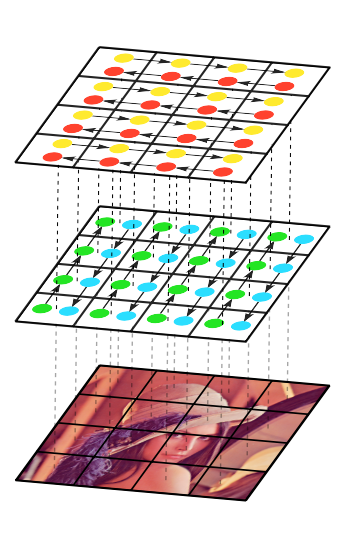
\includegraphics[width=0.5\textwidth]{img/ReNet.png}
	\caption{Schemat działania warstwy sieci ReNet.} Źródło: https://arxiv.org/abs/1505.00393
	\label{fig:ReNet-single-layer}
\end{figure}

Sieci ReNet \cite{DBLP:journals/corr/VisinKCMCB15} są alternatywą dla sieci konwolucyjnych w zadaniu rozpoznawania obrazów. Warstwy konwolucyjne realizują operację nakładania maski na tensor wejściowy, przez co informacje na wyjściu warstwy mają charakter lokalny. Sieć konwolucyjna w normalnym przypadku nie jest w stanie wykorzystać w pojedynczej warstwie informacji na temat całego obrazu. ReNet jest sposobem na zaadresowanie tej kwestii poprzez wykorzystanie sieci rekurencyjnej do obliczania aktywacji warstwy sieci z wykorzystaniem informacji zawartej w całym obrazie.

Każda warstwa ReNet składa się z czterech sieci rekurencyjnych, które skanują obraz w czterech kierunkach: z góry na dół, od dołu do góry, z lewej do prawej oraz z prawej do lewej (rys. \ref{fig:ReNet-single-layer}). Wejściem każdej z sieci jest zbiór pikseli o niewielkich rozmiarach rozmiarach (ang. patch). W każdym kroku aktywacja warstwy ReNet jest obliczana na podstawie poprzedniego stanu sieci i aktualnie analizowanego zbioru pikseli. 

Obraz wejściowy można zdefiniować jako:

\begin{equation}
	X = \{x_{i,j}\},\qquad X \in \mathbb{R}^{w \textrm{x} h \textrm{x} c}
\end{equation}

gdzie $w, h$ to rozmiary obrazu, a $c$ to liczba kanałów dla każdego piksela obrazu. Liczbę patchy w pojedynczym wierszu i kolumnie obrazu wejściowego można zatem zapisać jako:

\begin{gather}
	I=\frac{w}{w_p} \\
	J=\frac{h}{h_p} \nonumber
\end{gather}

gdzie $w_p$ i $h_p$ to wysokość i szerokość patha. Zbiór wszystkich patchy obrazu wejściowego jest dany jako: $P = \{p_{i,j}\}, P \in \mathbb{R}^{w_p \textrm{x} h_p \textrm{x} c}$. Pionowe przejście sieci po wszystkich patchach obrazu można zapisać jako funkcję aktywacji sieci rekurencyjnej:

\begin{gather}
    v_{i,j}^{F} = f_{VFWD} (v_{i,j-1}^F, p_{i,j}), \\
    v_{i,j}^{R} = f_{VREV} (v_{i,j+1}^R, p_{i,j}), \nonumber
\end{gather}

gdzie $f_{VFWD} (v_{i,j-1}^F, p_{i,j})$ to aktywacja sieci rekurencyjnej lub aktywacja komórki LSTM lub GRU. Wyjście po przejściu pionowym stanowi tensor $V = \{v_{i,j}\}_{i=1,...,I}^{j=1,...,J}$, będący mapą cech. Każdy element wyjścia $v_{i,j} \in \mathbb{R}^{2d}$ stanowi konkatenację aktywacji przejścia z góry na dół i z dołu na górę, gdzie $d$ to liczba jednostek rekurencyjnych wykorzystanych dla jednego patcha. Tensor $V$ jest wejściem dla drugiego elementu warstwy sieci realizującego przejście poziome. Operacja przejścia poziomego jest zdefiniowana analogicznie przez obliczenie aktywacji $f_{HFWD}, f_{HREV}$. Wynikiem tej operacji jest tensor $H = \{h_{i,j}\}$. 

Ostatecznie przekształcenie $\Phi$ realizowane przez całą warstwę sieci może zostać zapisane z wykorzystaniem wprowadzonych oznaczeń jako:

\begin{equation}
	\Phi: X \rightarrow V \rightarrow H
\end{equation}

\begin{figure}
\centering
	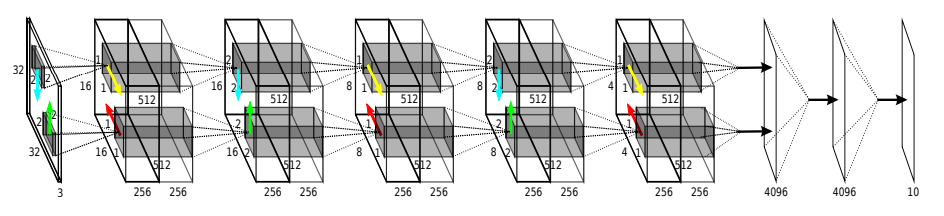
\includegraphics[width=0.9\textwidth]{img/ReNetArch.png}
	\caption{Schemat przepływu informacji w sieci ReNet.} Model ten został wykorzystany przez twórców architektury dla zbioru SVHN. Powyższy schemat przedstawia sieć z trzema warstwami ReNet, dwoma w pełni połączonymi warstwami oraz warstwą softmax. Każda warstwa ReNet składa się z dwóch etapów: sieci skanujących obraz w kierunku góra-dół, dół-góra oraz lewo-prawo, prawo-lewo. Rozmiar patchy sieci w każdej warstwie wynosi 2x2. Warto zauważyć, że rozmiar patchy przy skanowaniu sieci w kierunku poziomym musi wynosić 1x1, aby aktwacje obliczane przy przejściu poziomym dotyczyły tej samej części obrazu co przy przejściu pionowym (w trakcie przejścia pionowego patch o rozmiarze 2x2xc zostaje zamieniony na aktywacje sieci 1x1xd, gdzie d to liczba neuronów w warstwie). Liczba neuronów sieci rekurencyjnej dla pojedynczego przejścia wynosi 256. Aktywacje każdego neuronu ukrytego są łączone dla przejść w przeciwnych kierunkach, więc wyjście po dwóch przejściach jest tensorem o rozmiarach $I,J,2d$. W każdej warstwie następuje zmniejszenie wymiarów obrazu, co powoduje brak konieczności stosowania poolingu po warstwie ReNet. Warstwy w pełni połączone zawierają 4096 neuronów i wykorzystują funkcję aktywacji ReLu. Źródło: https://arxiv.org/abs/1505.00393
	\label{fig:ReNet}
\end{figure}

Każda kolejna warstwa sieci ReNet korzysta z wyjścia poprzedniej warstwy. Schemat działania sieci dla przykładowego zbioru danych, wraz z omówieniem realizowanych operacji został przedstawiony na rysunku \ref{fig:ReNet}.

\section{Krzywe wypełniające przestrzeń}

\section{Proponowana architektura sieci}



\chapter{Przeprowadzone badania}

\section{Metodyka badań}

\section{Reprodukcja wyników architektury ReNet}

Pierwszym eksperymentem jaki wykonano było zreprodukowanie wyników z \cite{DBLP:journals/corr/VisinKCMCB15}. Celem reprodukcji było potwierdzenie przesłanki do badań oraz sprawdzenie poprawności przygotowanej implementacji ReNet. W niniejszej sekcji podano krótki opis stosowanej metodyki i uzyskane wyniki.

\subsection{Statystyczna ewaluacja wyników}

Reprodukcja badań nie stanowi zasadniczej części badań. Z tego względu uproszczono proces zbierania wyników. Podane rezultaty są wynikiem pojedynczego procesu uczenia, bez powtarzania prób. W \cite{tom-mitchell-machine-learning} podano sposób analizy błędu pojedynczego pomiaru skuteczności algorytmu.

Dysponując zbiorem danych $d$ wylosowanym z pewnego nieznanego rozkładu $\mathcal{D}$ chcemy oszacować rzeczywisty błąd $err_{\mathcal{D}}$ popełniany przy przez hipotezę $h$ dla dowolnego datasetu wylosowanego z $\mathcal{D}$. Błąd popełniony na datasetcie $err_d$, dany jest wzorem:

\begin{equation}
	err_d = \frac{t}{n}
\end{equation}

Przy założeniu, że $d$ zawiera próbki niezależne od siebie oraz od $h$ i liczba przykładów uczących $n$ w zbiorze uczącym $d$ jest większa od 30, $err_d$ jest najlepszym estymatorem $err_{\mathcal{D}}$. Przedział w którym wartość $err_{\mathcal{D}}$ znajduję się z prawdopodobieństwem około 95\% można wyznaczyć jako:

\begin{equation}
	err_{d} \pm 1.96 \sqrt{\frac{err_{d}(1 - err_{d})}{n}} 
\end{equation}

Przedziały te zostały podane wraz z uzyskanymi w trakcie reprodukcji badań wartościami skuteczności na zbiorze testowym.

\section{Opis eksperymentu}

\subsection{Zbiór danych}

\subsection{Wykorzystane narzędzia i hardware}

\subsection{Dobór hiperparametrów modelu}



\chapter{Wyniki}


\chapter{Wnioski}

\bibliography{bibliography}

\listoffigures

\end{document}